\documentclass{main}
\begin{document}
\section{Tor - Onion Routing}

Tor, short for "The Onion Router," is free and open-source software for enabling anonymous communication. It directs Internet traffic via a free, worldwide, volunteer overlay network that consists of more than seven thousand relays.
Although Tor was initially developed by the US government in 2002, it is not presently controlled by any one entity.
Tor has been one of the most famous and widely used anonymous communication tool.
The release of the Tor Browser made Tor more accessible to everyday internet users and activists.  
Tor Browser is simply an Internet Browser based on Firefox, with modifications to hide the user's IP address. 

\subsection{Onion Routing}

\begin{wrapfigure}{l}{0.5\textwidth}
    \centering
    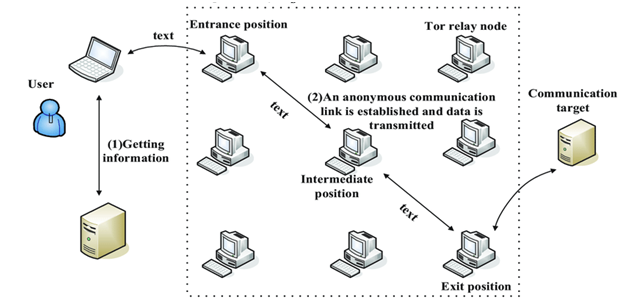
\includegraphics[width=0.5\textwidth]{Resources/images/onion-routing.png}
\end{wrapfigure}

In a nutshell, onion routing refers to encapsulating message under layers of encryption at different nodes before it reaches the final destination. 
All the nodes only know about the previous node and the next node. 
In this way, no single node knows the entire path of the message. 
Clients choose these path randomly and build a circuit. 
These circuits change every few minutes preventing any snooping attempts. 

\subsection{The Tor Design}

\subsubsection{Onion Router}
Each onion router runs as a normal user-level process.
It maintains a TLS connection to every other onion router in the network.
The task of an onion router is to connect to requested destination and relay the data. 
Each onion router knows only the previous and next onion router in the circuit.
Each onion router maintains a long-term identity key and a short-term onion key.
The identity key is used to sign TLS certificates and to sign the router descriptor.
Router descriptor is a summary of its keys, address, bandwidth, exit policy, and so on.
Directory servers use identity key to sign directories. 
The onion key is used to decrypt requests from users to set up a circuit and negotiate ephemeral keys.

\subsubsection{Onion Proxy}
Each user runs a Tor client called an Onion Proxy on their computer. 
The Onion Proxy is responsible to fetch directories, building circuits, and sending messages through the circuits. 
These onion proxies accept TCP streams and multiplex them across the circuits.

\subsubsection{Cells}

Onion routers communicate with one another, and with users Onion Proxies, via TLS connections with ephemeral keys. 
Traffic passes along these connections in fixed-size cells.
Each cell is 512 bytes, and consists of a header and a payload.

\begin{figure}[h]
	\centering
	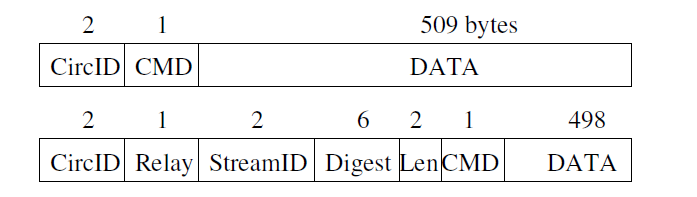
\includegraphics[width=0.7\textwidth]{Resources/images/tor_cell.png}
\end{figure}

\begin{description}
    \item [CircID] is different for each hop (OP/OR or OR/OR) in the circuit.
    \item [CMD] specifies the type and action of the cell.

    \item [CONTROL] cells are used to manage circuits and connections. These are interpretted directly by the node receiving it. Some of the control cells command are create, created, destroy, padding, etc.
    % \begin{itemize}
    %     \item CREATE/CREATED: request/response to create a new circuit
    %     \item DESTROY: to teardown a circuit
    %     \item PADDING: currently used for keepalive
    % \end{itemize}
    \item [RELAY] cells carry end-to-end stream data. They have additional header fields to specify the stream ID, a checksum to maintain integrity, length of the relay payload and a relay command. Some of relay cell commands are relay begin, relay data, relay end, relay teardown, etc.
\end{description}
        
\subsubsection{Circuits and streams}  
A circuit is a path through the Tor network.
Each circuit can be shared by many TCP streams.
These circuits are built periodically by client's OP and are torn down after their expiry.
Each stream is a sequence of relay cells traveling along a circuit.

\subsubsection{Directory Servers}

Tor uses a small group of redundant, well-known onion
routers to track changes in network topology and node state,
including keys and exit policies. Each such directory server
acts as an HTTP server, so clients can fetch current network
state and router lists, and so other ORs can upload state information. Onion routers periodically publish signed statements
of their state to each directory server. The directory servers
combine this information with their own views of network
liveness, and generate a signed description (a directory) of
the entire network state. Client software is pre-loaded with a
list of the directory servers and their keys, to bootstrap each
client's view of the network.

\subsubsection{Rendezvous Points and hidden services}
Rendezvous points are a building block for location-hidden
services. Location-hidden services allow a person to offer a TCP service, such as a webserver, without revealing his IP address.

\subsection{Constructing a Circuit}

A user's OP constructs circuits incrementally, negotiating a symmetric key with each OR on the circuit, one hop at a time.
To create a circuit, the OP (call her Alice) sends a CREATE cell to an OR of her choice (call him Bob) on the circuit containing the first half of a Diffie-Hellman handshake encrypted using OR's public key.
The OR replies with a CREATED cell containing the second half of the handshake and a hash of the negotiated key.
Further comunication between them is encrypted using the negotiated key.

To extend the circuit further, ALice sends a relay EXTEND cell to Bob, containing the address of the next OR and the first half of a new Diffie-Hellman handshake encrypted using that OR's public key.
Bob copies the first half of the handshake into a CREATE cell and sends it to the next OR.
When the next OR replies with a CREATED cell, Bob wraps into relay extended cell and pass it back to Alice.

\begin{figure}[h]
    \centering
    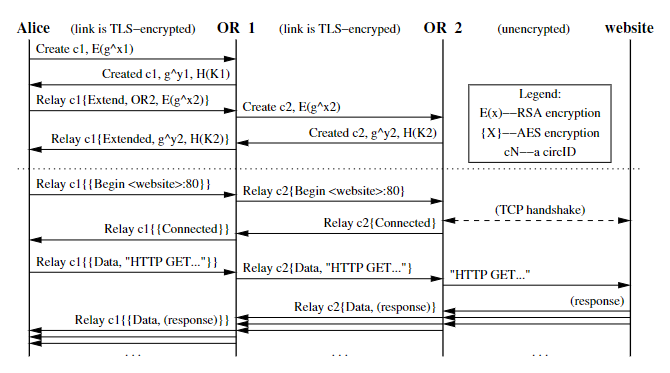
\includegraphics[width=0.8\textwidth]{Resources/images/tor_circuit.png}
\end{figure}

This circuit-level handshake protocol achieves unilateral entity authentication.

\subsection{Role of Relay Cells}
Upon re-ceiving a relay cell, an OR looks up the corresponding circuit,
and decrypts the relay header and payload with the session
key for that circuit. If the cell is headed away from Alice the
OR then checks whether the decrypted cell has a valid digest.
If valid, it accepts the relay cell and processes it as described
below. Otherwise, the OR looks up the circID and OR for the
next step in the circuit, replaces the circID as appropriate, and
sends the decrypted relay cell to the next OR.

OPs treat incoming relay cells similarly: they iteratively
unwrap the relay header and payload with the session keys
shared with each OR on the circuit, from the closest to farthest. If at any stage the digest is valid, the cell must have
originated at the OR whose encryption has just been removed.

To construct a relay cell addressed to a given OR, Alice assigns the digest, and then iteratively encrypts the cell payload
(that is, the relay header and payload) with the symmetric key
of each hop up to that OR.

When an OR later replies to Alice with a relay cell, it encrypts the cell's relay header and payload with the single key
it shares with Alice, and sends the cell back toward Alice
along the circuit. Subsequent ORs add further layers of en-
cryption as they relay the cell back to Alice.

To tear down a circuit, Alice sends a destroy control cell.
Each OR in the circuit receives the destroy cell, closes all
streams on that circuit, and passes a new destroy cell forward.
These circuits can also be torn down incremently using relay truncate cell.

\subsection{Rendezvous points in Tor}

\begin{figure}[h]
    \centering
    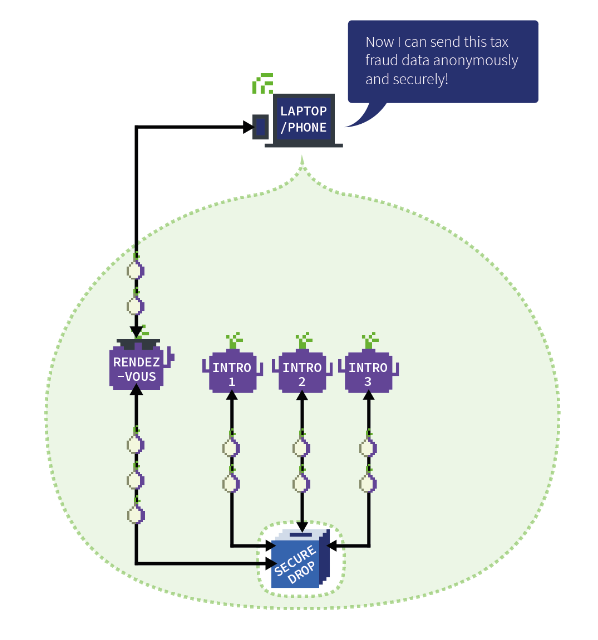
\includegraphics[width=0.5\textwidth]{Resources/images/onion_services.png}
\end{figure}

The following steps are performed on behalf of Alice and Bob by their local OPs to communicate using a rendezvous point:


\begin{itemize}
    \item Bob generates a long-term public key pair to identify his
    service.
    \item Bob chooses some introduction points, and advertises
    them on the lookup service, signing the advertisement
    with his public key. He can add more later.
    \item Bob builds a circuit to each of his introduction points,
    and tells them to wait for requests.
    \item Alice learns about Bob's onion service out of band. She retrieves
    the details of Bob's service from the lookup service. If
    Alice wants to access Bob's service anonymously, she
    must connect to the lookup service via Tor.
    \item Alice chooses an OR as the rendezvous point (RP) for
    her connection to Bob's service. She builds a circuit
    to the RP, and gives it a randomly chosen “rendezvous
    cookie” to recognize Bob.
    \item Alice opens an anonymous stream to one of Bob's intro-
    duction points, and gives it a message (encrypted with
    Bob's public key) telling it about herself, her RP and ren-
    dezvous cookie, and the start of a DH handshake. The
    introduction point sends the message to Bob.
    \item If Bob wants to talk to Alice, he builds a circuit to Al-
    ice's RP and sends the rendezvous cookie, the second
    half of the DH handshake, and a hash of the session key
    they now share.
    \item The RP connects Alice's circuit to Bob's. Note that RP
    can't recognize Alice, Bob, or the data they transmit.
    \item Alice sends a relay begin cell along the circuit. It arrives
    at Bob's OP, which connects to Bob's webserver.
    \item An anonymous stream has been established, and Alice
    and Bob communicate as normal.

\end{itemize}



\end{document}
